\chapter{\IfLanguageName{dutch}{Proof of concept}{Proof of concept}}%
\label{ch:proofofconcept}

\section{Gekozen technologieën}

\subsection{Framework}

Gezien de expertise van we are, is er voor het platform gekozen voor een responsive React\footnote{\href{https://react.dev/}{https://react.dev/}}-website. Hiervoor is gebruik gemaakt van TypeScript \footnote{\href{https://www.typescriptlang.org/}{https://www.typescriptlang.org/}}.

Voor de implementatie van authenticatie is er gebruik gemaakt van Auth0\footnote{\href{https://auth0.com/}{https://auth0.com/}}. De redenen waarom er voor Auth0 gekozen is, zijn: de mogelijkheid om aan te melden met een Google-account, makkelijke integratie in React en de mogelijkheid tot een gratis abonnement wanneer het aantal gebruikers onder de 7000 blijft, wat voor deze POC meer dan voldoende is.

\subsection{Component libraries}
Gezien de korte ontwikkeltijd die beschikbaar was, zijn Material UI Core\footnote{\href{https://mui.com/core/}{https://mui.com/core/}} en Material UI X\footnote{\href{https://mui.com/x/}{https://mui.com/x/}} component libraries gebruikt voor de ontwikkeling van deze website, om zo het ontwikkelproces te vergemakkelijken. Er is gekozen voor Material UI door diens universele look-and-feel, het ruime aanbod aan gratis componenten en de beschikbaarheid van grafische componenten. Daarnaast zijn deze componenten uitermate geschikt voor zowel mobiel als desktop gebruik.

\subsection{Databank}

Deze applicatie gebruikt een graafdatabank, meer specifiek Neo4J\footnote{\href{https://neo4j.com/}{https://neo4j.com/}}. Er is in deze situatie gekozen voor een graaf databank omdat het zeer simpel op te zetten is en er geen databank-schema ontworpen moet worden, wat het dus zeer simpel maakt om snel te ontwikkelen en gaandeweg eventueel zaken aan te passen indien nodig.

\section{Opbouw van de applicatie}

De applicatie is opgesteld op basis van de volgende bouwstenen: een centraal dashboard, een overzicht van eigen prestaties, een oplijsting van de teamleden en een profielpagina.

\subsection{Dashboard}
Op het dashboard is de meeste informatie te zien: zowel persoonlijke evolutie over één week en over drie weken als de team en persoonlijke ranking zijn er te vinden. Om kleinere teams evenveel kans te geven, houdt de teamranking rekening met de grote van het team bij de berekening.

\subsection{Persoonlijk overzicht}
Op het persoonlijk overzicht is een lijst van de gepresteerde activiteiten te zien (figuur \ref{fig:performances} en figuur \ref{fig:performancesMobile}), en kunnen gebruikers ook hun prestaties ingeven. Hier is voldoende ruimte voorzien voor de ingave van technische gegevens, zoals gemiddelde hartslag en hoogtemeters. Afhankelijk van het type activiteit, en wanneer een afstand en duur ingegeven zijn, berekent de applicatie ook een gemiddelde snelheid. Zo kunnen frequente sporters eventueel een vooruitgang opmerken.

\begin{figure}[h]
    \caption[Overzicht activiteiten website]{Overzicht van gepresteerde activiteiten in de applicatie, gezien vanop een laptop.}
    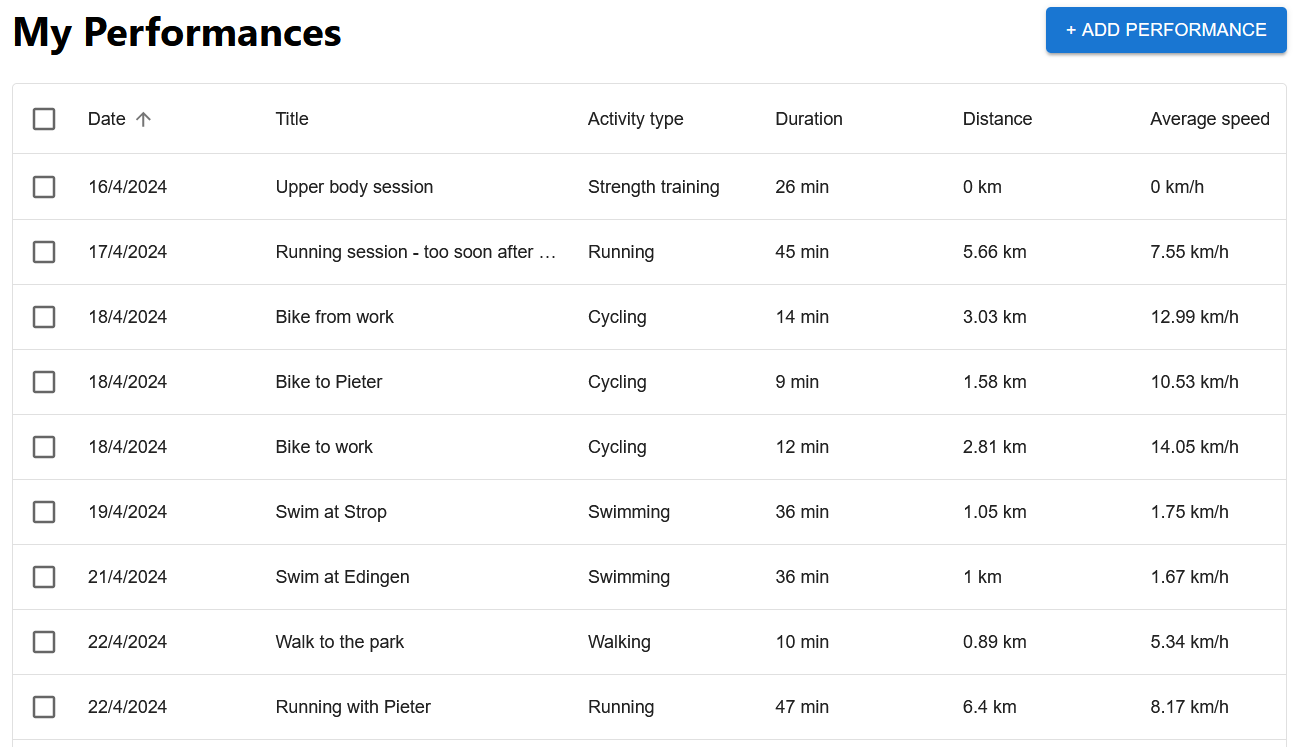
\includegraphics[width=1\textwidth]{MyPerformances}
    \label{fig:performances}
\end{figure}

\begin{figure}[h]
    \caption[Overzicht activiteiten website smartphone]{Overzicht van gepresteerde activiteiten in de applicatie, gezien vanop een smartphone.}
    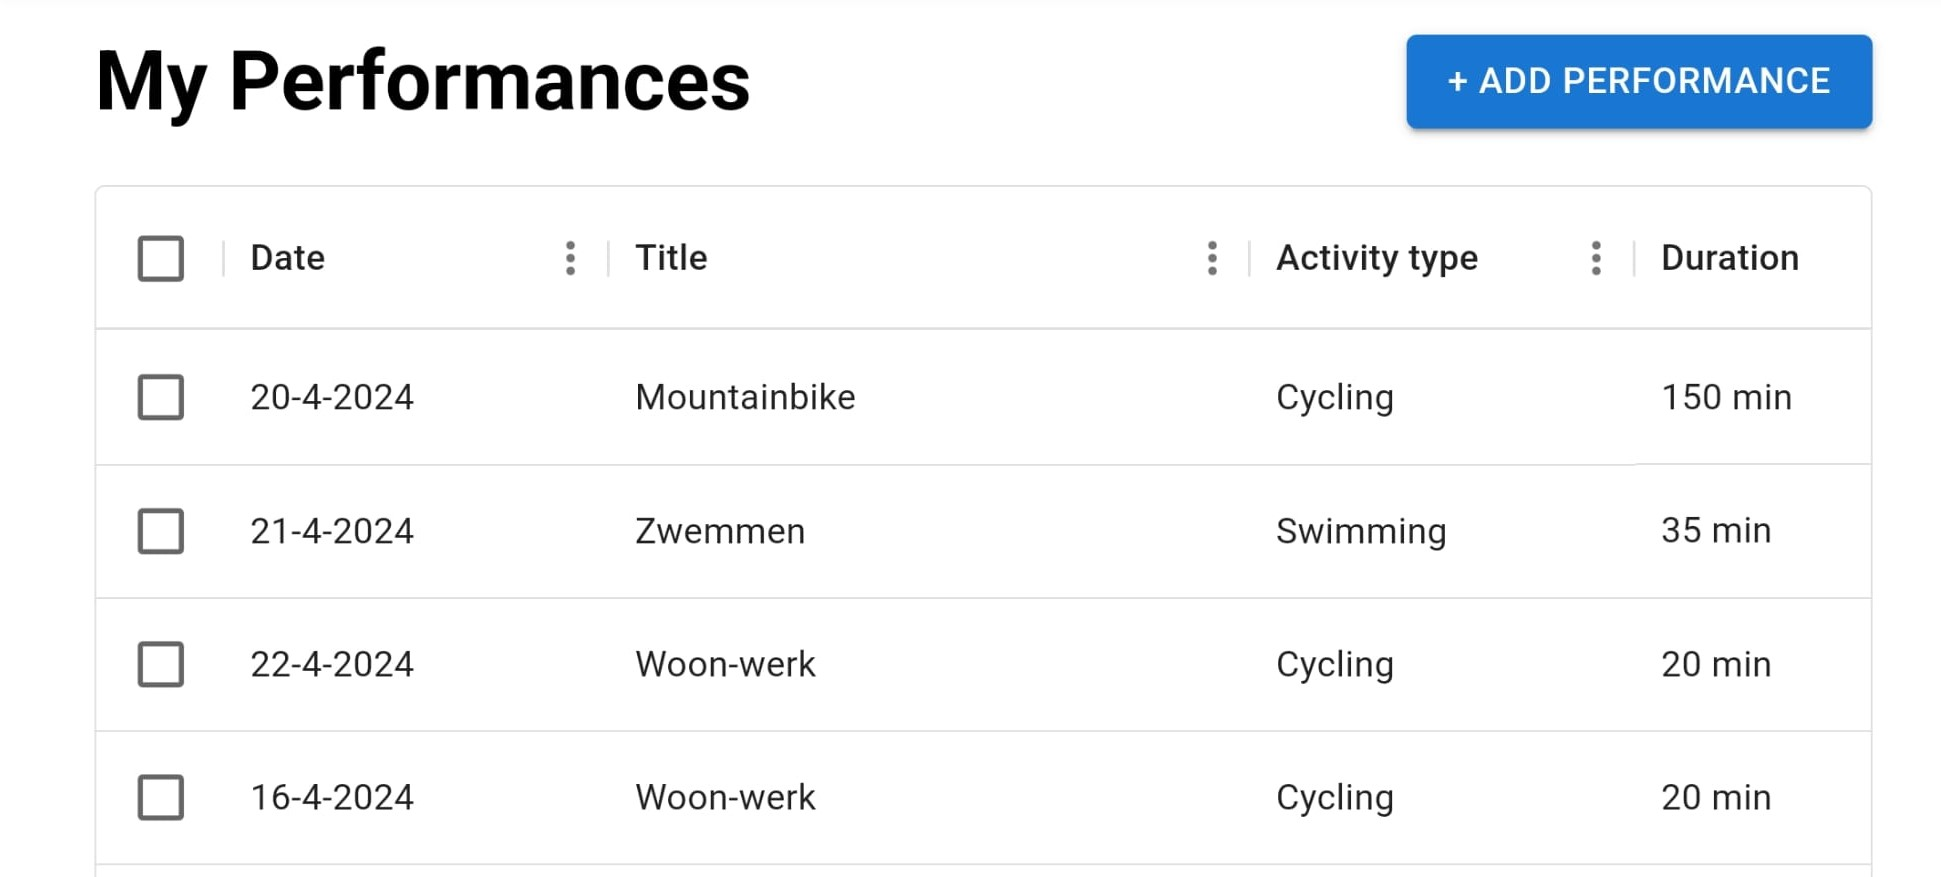
\includegraphics[width=1\textwidth]{MyPerformancesMobile}
    \label{fig:performancesMobile}
\end{figure}

\subsection{Teamoverzicht}

Dit overzicht is een simpele oplijsting van alle teamleden waartoe de aangemelde gebruiker behoort.

In de toekomst zou dit uitgebreid kunnen worden met een overzicht van de prestaties van een team, zodat er ook binnen een team gamification speelt en wat mogelijks tot meer motivatie kan leiden.

\subsection{Profiel pagina}

Op deze pagina kan een gebruiker een avatar, team en naam kiezen waarmee die weergegeven wordt.